\chapter{Inferenza della struttura}
\section{Analisi delle tecniche utilizzate}
\label{sec:misure}
Il nostro obiettivo principale è quello di verificare se sia possibile apprendere la struttura della rete a partire da un dataset contenente i dati di $10000$ pazienti con la sindrome del \textit{BlueBaby}. Al fine di fare ciò, sono state considerate due differenti approcci, ovvero la tecnica \texttt{Hill Climb} e la tecnica \texttt{Tabù Search}. Entrambe le tecniche di analizzate sono basate su un processo meta-euristico di ottimizzazione di una funzione di score. Documentandoci sulle due tecniche prese in esame, ed effettuando alcuni test preliminari, abbiamo notato come le performance della ricerca Tabù siano superiori a quelle della prima tecnica citata, in quanto la seconda permette di evitare lo stallo della ricerca nei minimi locali.\\
\begin{table}[t!]
	\centering
	\caption{Differenti funzioni di score a confronto. La colonna \textit{Archi paper} mostra il numero di archi presenti nella rete proposta dal paper ma non presente nel modello generato. Viceversa, l'ultima colonna indica il numero di archi presenti nel modello appreso ma non presenti nella rete del paper.}
	\begin{tabular}{|c|c|c|c|c|}
		\hline 
		Funzione & Archi generati  & Archi comuni & Archi paper & Archi appreso \\ 
		\hline 
		aic & 32 & 24 & 1 & 8 \\ 
		\hline 
		bic & 26 & 18 & 7 & 8 \\ 
		\hline 
		bde & 26 & 21 & 4 & 5 \\ 
		\hline 
		bds & 26 & 18 & 7 & 8 \\ 
		\hline 
		mbde & 26 & 21 & 4 & 5 \\ 
		\hline 
		bdla & 26 & 21 & 4 & 5 \\ 
		\hline 
		k2 & 25 & 24 & 1 & 1 \\ 
		\hline 
	\end{tabular} 
	\label{tab:score}
\end{table}
Abbiamo quindi approfondito le possibili funzioni di score disponibili per la ricerca Tabù, confrontando la rete prodotta con quella fornita dal \textit{paper} di riferimento. I risultati ottenuti, proposti in Tabella \ref{tab:score}, mostrano come molte misure ottengano performance simili, mentre quella che si distingue dalle altre risulta essere la funzione \texttt{k2}, che stima correttamente il numero di archi, inserendo un solo arco in posizione non ottimale.

La Figura mostra la rappresentazione prodotta dall'algoritmo \texttt{Tabù Search} con la funzione di score \texttt{k2}; confrontando questa struttura con quella proposta in Figura \ref{fig:paperstructure}, notiamo come l'unico arco differente sia quello che collega i nodi \textit{Age} e \textit{Sick}.

\begin{figure}
	\centering
	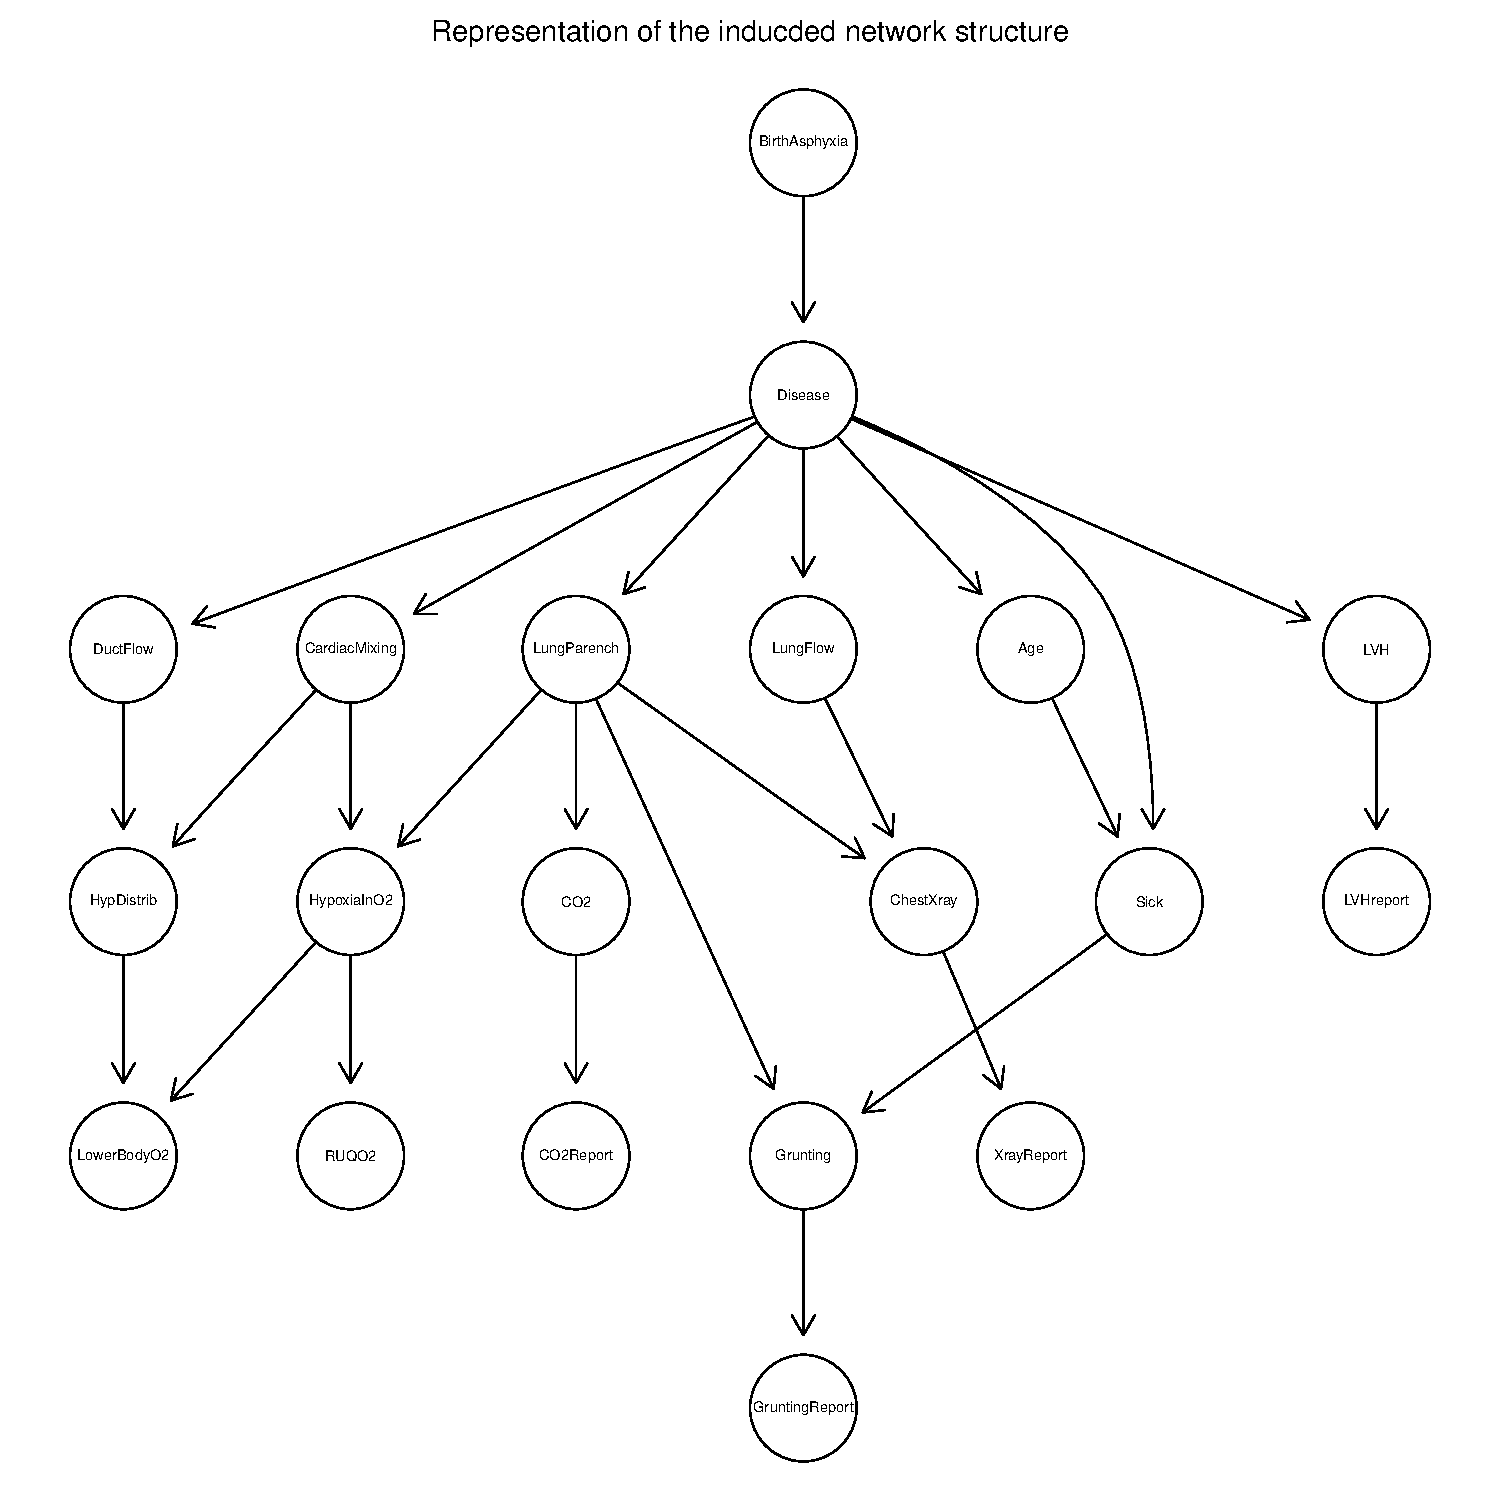
\includegraphics[width=.9\linewidth]{images/induced_structure}
	\caption{Rappresentazione della struttura appresa con la ricerca di Tabù e la funzione di score \texttt{k2}}
	\label{fig:inducedstructure}
\end{figure}

\newpage
\section{Misure di performance delle reti}
Una volta indotta la struttura della rete con il metodo illustrato nella Sezione \ref{sec:misure}, abbiamo deciso di valutare le capacità predittive della reti proposte per quanto riguarda la predizione della variabile \textit{Disease}. Per fare ciò, abbiamo deciso di effettuare un'operazione di \textit{10-times 10-fold coross validation}, al fine di garantire la significatività statistica dei risultati ottenuti. In ogni fold, per le due reti vengono stimate le CPT di ogni nodo utilizzando il $90\%$ del dataset; viene poi utilizzata la tecnica \textit{likelihood weighting}, generando 500 sample per ogni nuova osservazione, per determinare il valore del nodo \textit{Disease} associato ad una particolare istanza.

Le performance ottenute, riportate nelle Figure \ref{fig:paperperformance} e \ref{fig:inducedperformance}, calcolate come la media delle dieci ripetizioni del processo di \textit{cross validation}, risultano essere molto simili. Al fine di indagare se le performance dei due modelli proposti fossero statisticamente differenti, sono stati eseguiti dei test di significatività \textit{t-student}; i risultati ottenuti hanno mostrato come le performance medie dei due modelli siano di fatto equivalenti, a meno di un errore attribuibile al caso.
\begin{figure}
	\centering
	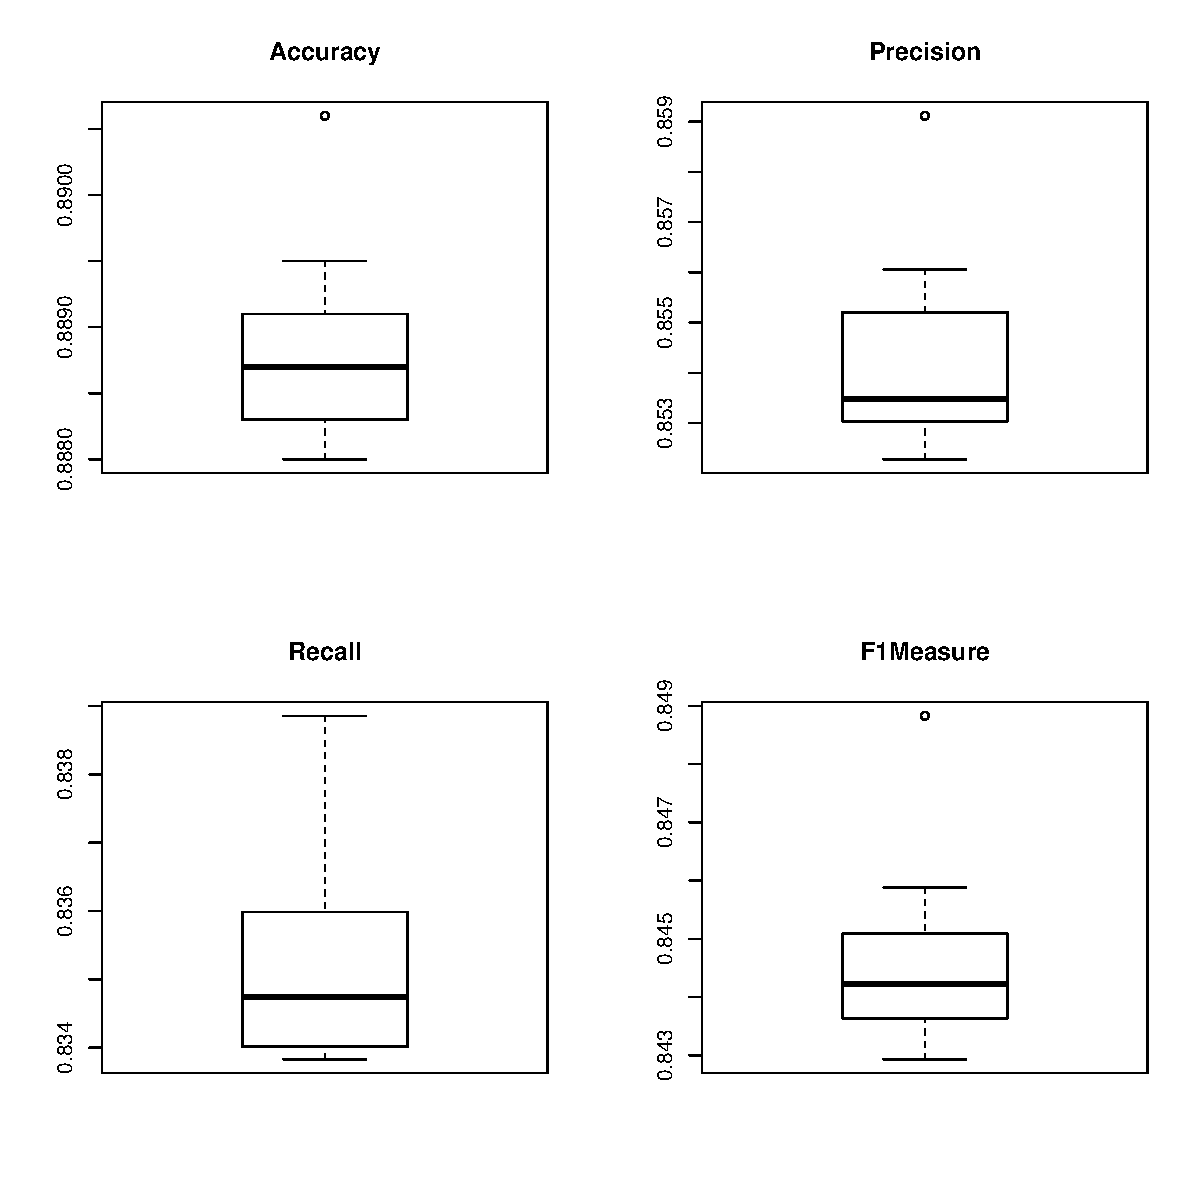
\includegraphics[width=0.7\linewidth]{images/paper_performance}
	\caption{Performance ottenute dalla rete proposta dal paper.}
	\label{fig:paperperformance}
\end{figure}
\begin{figure}
	\centering
	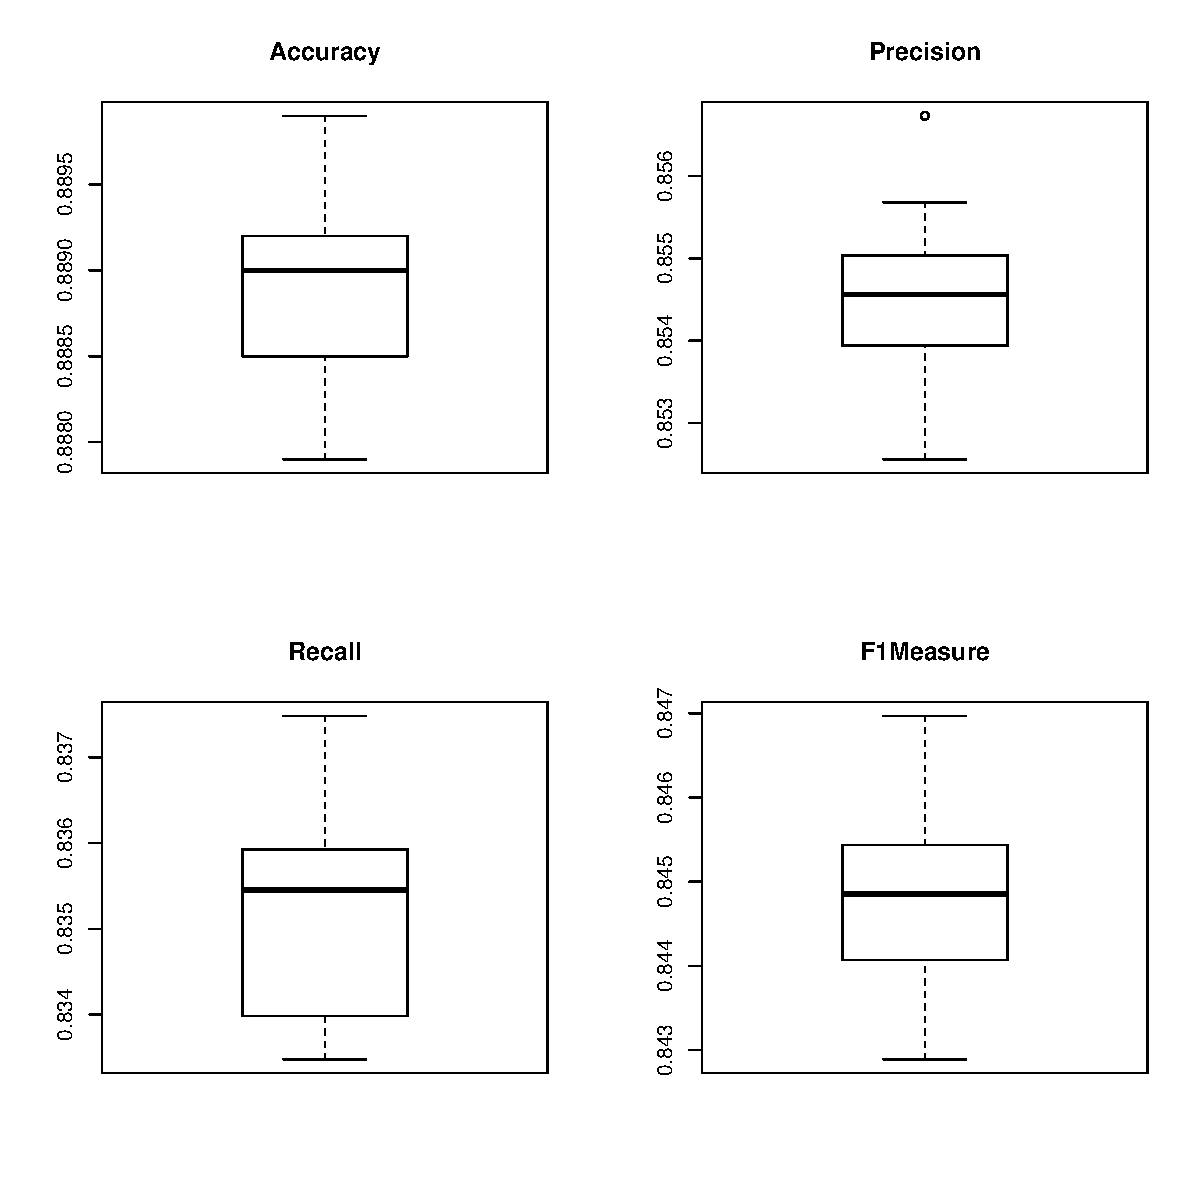
\includegraphics[width=0.7\linewidth]{images/induced_performance}
	\caption{Performance ottenute dalla rete appresa dal dataset.}
	\label{fig:inducedperformance}
\end{figure}
Questo è una conferma di come la struttura appresa dal dataset utilizzato sia valida e in grado di predire valori per il nodo \textit{Disease} in modo efficace; la presenza di un'unico arco in posizione differente non ha quindi impattato negativamente sulle performance predittive.

Analizzando più specificamente il dominio di applicazione, abbiamo deciso di ripetere le operazioni di inferenza del valore di \textit{Disease} fornendo non più un'evidenza completa delle variabili della rete, bensì fornendo solo di quei nodi che abbiamo ritenuto essere effettivamente osservabili dai medici, ovvero i dati del paziente e i risultati degli esami.\\
Le performance ottenute dalle due reti, riportate nelle Figure \ref{fig:paperperformancehalf} e \ref{fig:inducedperformancehalf}, sono, come ci aspettavamo, sensibilmente inferiori; ciononostante, le performance dei due modelli risultano nuovamente statisticamente non dissimili, avallando ulteriormente la tesi che la struttura appresa dai dati sia valida.\\
\begin{figure}
	\centering
	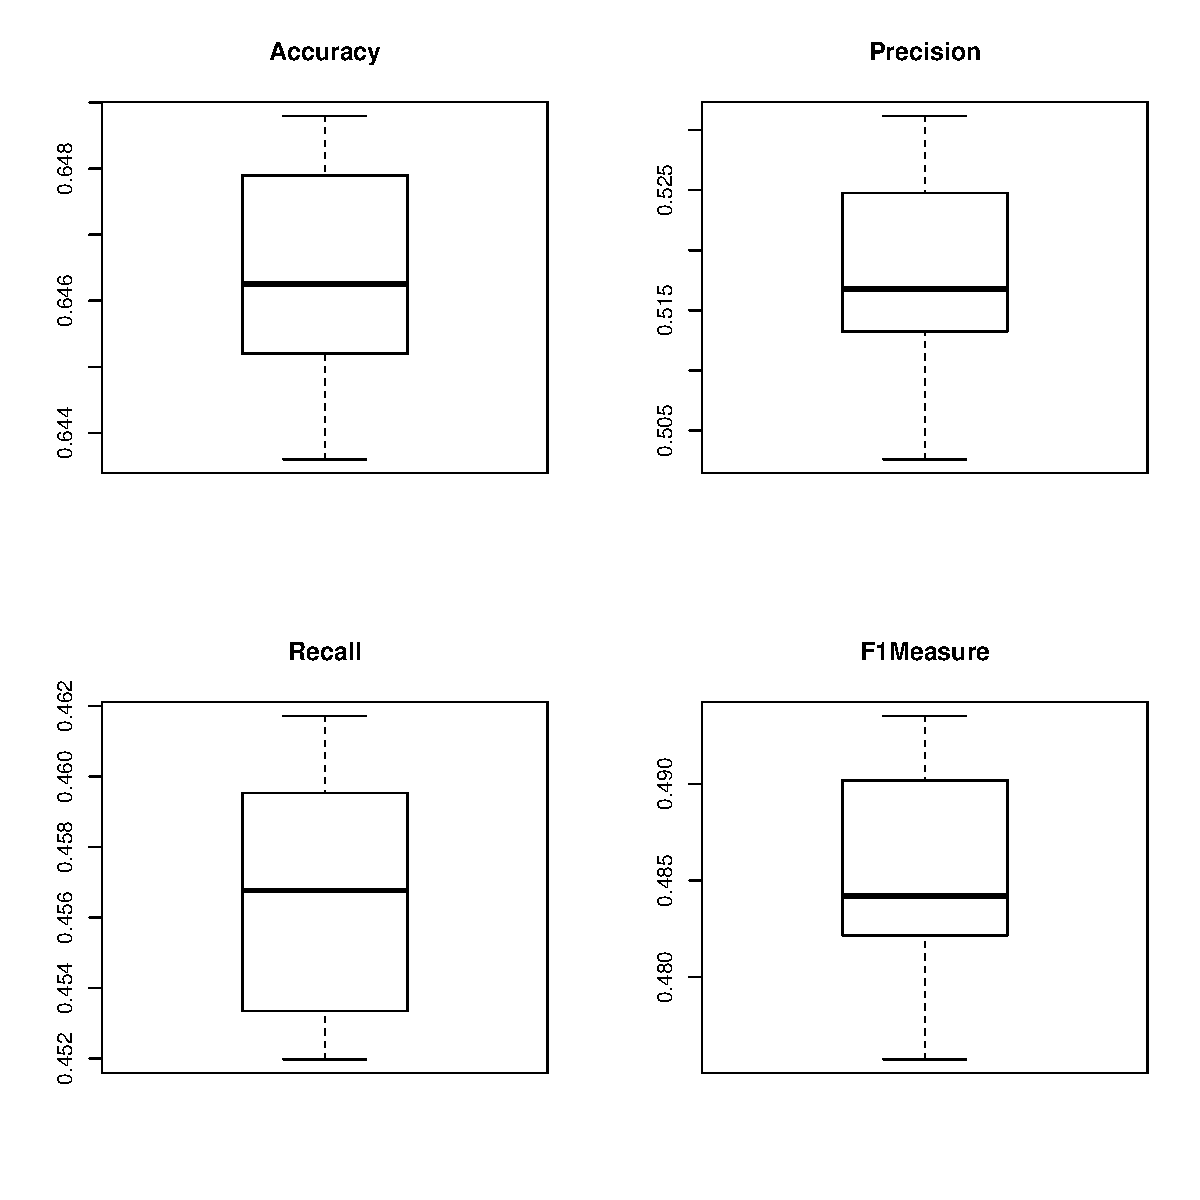
\includegraphics[width=0.7\linewidth]{images/paper_performance_half}
	\caption{Performance ottenute dalla rete proposta dal paper.}
	\label{fig:paperperformancehalf}
\end{figure}
\begin{figure}
	\centering
	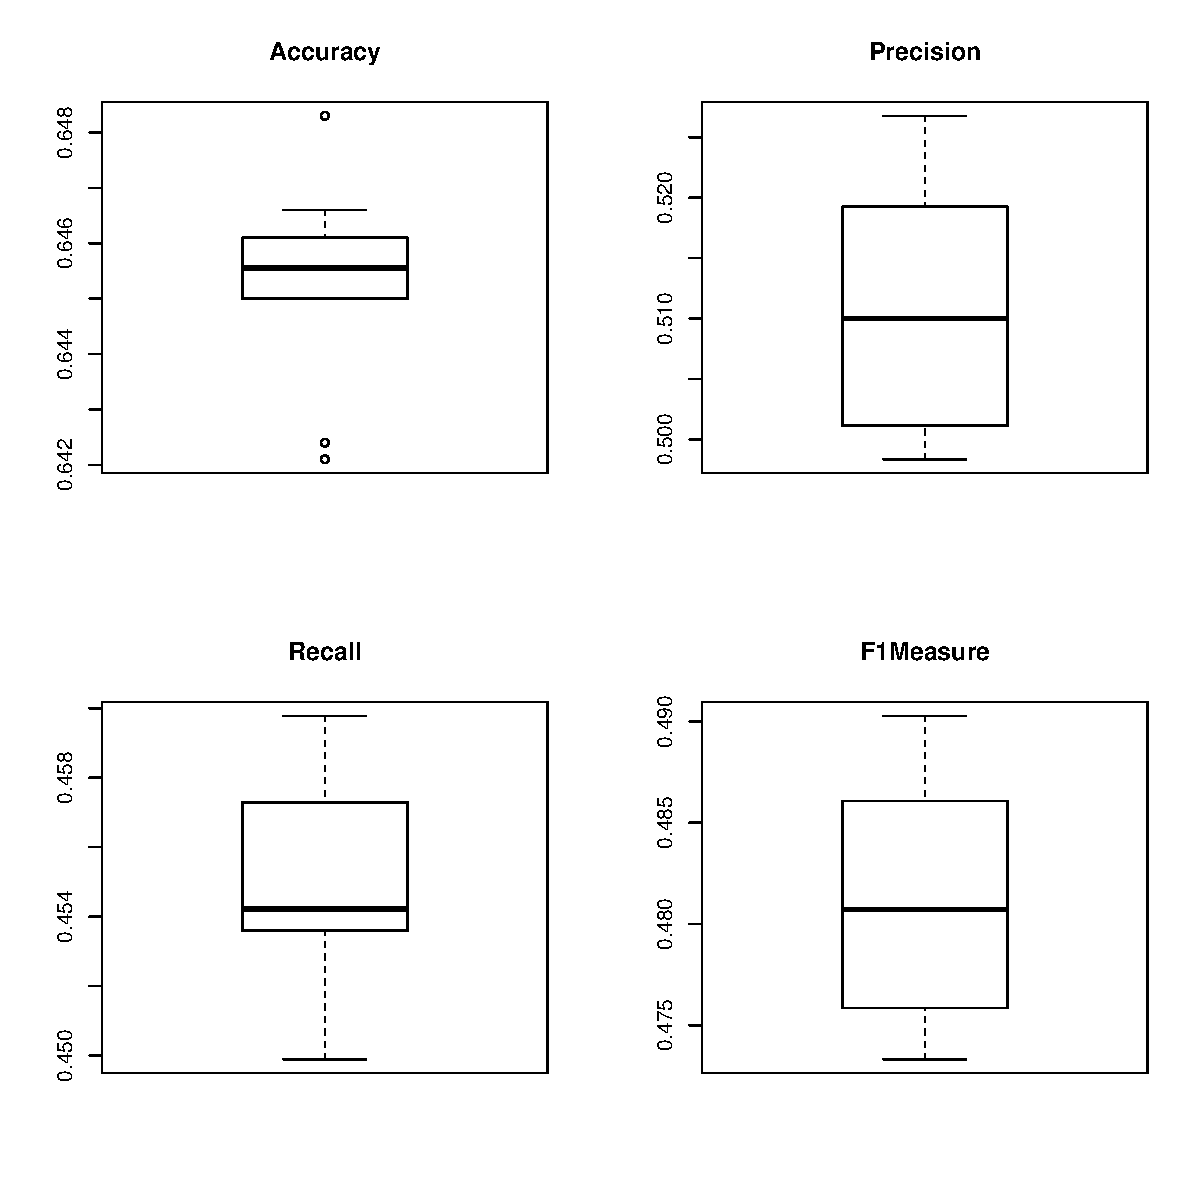
\includegraphics[width=0.7\linewidth]{images/induced_performance_half}
	\caption{Performance ottenute dalla rete appresa dal dataset.}
	\label{fig:inducedperformancehalf}
\end{figure}


